\documentclass[11pt,a4paper]{report}

% =====================================================
% PACKAGES ET MISE EN PAGE
% =====================================================
\usepackage[utf8]{inputenc}
\usepackage[T1]{fontenc}
\usepackage[french]{babel}
\usepackage{mathpazo}
\usepackage[scaled=0.95]{helvet}
\usepackage[final]{microtype}
\usepackage{geometry}
\geometry{top=2.7cm,bottom=2.7cm,left=2.4cm,right=2.4cm}
\usepackage{setspace}
\setstretch{1.18}
\usepackage{graphicx}
\usepackage[table]{xcolor}
\usepackage{array,booktabs,longtable,tabularx}
\usepackage{enumitem}
\usepackage{titlesec}
\usepackage{fancyhdr}
\usepackage{listings}
\usepackage{tikz}
\usetikzlibrary{arrows.meta,positioning,shapes.geometric,fit}
\usepackage[most]{tcolorbox}
\usepackage{float}
\usepackage{caption}
\usepackage{subcaption}
\usepackage{pdflscape}
\usepackage{hyperref}
\usepackage{url}
\usepackage{amssymb}
\usepackage{pifont}
\usepackage{etoolbox}
\usepackage{ragged2e}
\usepackage{needspace}
\setlength{\headheight}{23pt}
\setlength{\parskip}{4pt}
\setlength{\parindent}{0pt}
\emergencystretch=2em
\raggedbottom

% =====================================================
% COULEURS
% =====================================================
\definecolor{mainblue}{RGB}{0,51,102}
\definecolor{accentblue}{RGB}{0,102,204}
\definecolor{softgray}{RGB}{245,247,250}
\definecolor{codebg}{RGB}{250,250,250}
\definecolor{alertred}{RGB}{190,45,45}
\definecolor{tealgreen}{RGB}{0,128,128}
\definecolor{darkgray}{RGB}{70,70,70}
\definecolor{lightyellow}{RGB}{255,250,230}
\definecolor{softgreen}{RGB}{232,247,239}
\definecolor{softred}{RGB}{252,236,236}

\newcommand{\cmark}{\ding{51}}
\newcommand{\xmark}{\ding{55}}

% =====================================================
% METADONNEES
% =====================================================
\newcommand{\ReportTitle}{Conception et mise en oeuvre d'une solution décisionnelle}
\newcommand{\ReportSubtitle}{Data Warehouse, ETL Pentaho PDI et tableaux de bord Power BI pour l'analyse de la santé mentale des adolescents}
\newcommand{\AuthorNames}{BEN ABDELLAH Mosab}
\newcommand{\Supervisor}{Pr. \textit{BADIR HASSAN}}
\newcommand{\Institution}{École Nationale des Sciences Appliquées de Tanger}
\newcommand{\Context}{Cycle ingénieur informatique -- Module Business Intelligence / Data Warehouse}
\newcommand{\AcademicYear}{Année universitaire 2025--2026}
\newcommand{\LogoLeft}{cropped-ensa.png}
\newcommand{\LogoRight}{images.png}

\hypersetup{
  colorlinks=true,
  linkcolor=mainblue,
  urlcolor=tealgreen,
  pdftitle={\ReportTitle},
  pdfauthor={\AuthorNames}
}

% =====================================================
% TITRES
% =====================================================
\titleformat{\chapter}[display]
  {\fontfamily{phv}\selectfont\huge\bfseries\color{mainblue}}
  {\flushright\fontsize{50}{50}\selectfont\color{gray!25}\thechapter}
  {-14pt}
  {\Huge}
  [\vspace{1ex}\titlerule]

\titleformat{\section}
  {\fontfamily{phv}\selectfont\Large\bfseries\color{mainblue}}
  {\thesection}{0.8em}{}

\titleformat{\subsection}
  {\fontfamily{phv}\selectfont\large\bfseries\color{accentblue}}
  {\thesubsection}{0.8em}{}

\captionsetup{font=small,labelfont=bf,textfont=it,width=0.92\linewidth}

% =====================================================
% EN-TETES SANS CHEVAUCHEMENT
% =====================================================
\pagestyle{fancy}
\fancyhf{}
\fancyhead[L]{\sffamily\footnotesize\color{darkgray} Projet BI -- DWH Mental Health}
\fancyhead[R]{\sffamily\footnotesize\color{mainblue} ENSA Tanger}
\fancyfoot[C]{\sffamily\footnotesize\thepage}
\renewcommand{\headrulewidth}{0.4pt}
\renewcommand{\headrule}{\hbox to\headwidth{\color{mainblue}\leaders\hrule height \headrulewidth\hfill}}
\fancypagestyle{plain}{%
  \fancyhf{}
  \fancyfoot[C]{\sffamily\footnotesize\thepage}
  \renewcommand{\headrulewidth}{0pt}
}

% =====================================================
% CODE
% =====================================================
\lstdefinestyle{sqlstyle}{
  language=SQL,
  backgroundcolor=\color{codebg},
  basicstyle=\ttfamily\small\color{black!85},
  keywordstyle=\color{blue!70!black}\bfseries,
  commentstyle=\color{gray}\itshape,
  stringstyle=\color{tealgreen},
  numbers=left,
  numberstyle=\tiny\color{gray!60},
  frame=none,
  breaklines=true,
  columns=fullflexible,
  showstringspaces=false,
  aboveskip=0pt,
  belowskip=0pt
}
\lstdefinestyle{plaincode}{
  backgroundcolor=\color{codebg},
  basicstyle=\ttfamily\small\color{black!85},
  numbers=left,
  numberstyle=\tiny\color{gray!60},
  frame=none,
  breaklines=true,
  columns=fullflexible,
  showstringspaces=false,
  aboveskip=0pt,
  belowskip=0pt
}
\lstset{inputencoding=utf8,extendedchars=true,literate={é}{{\'e}}1 {è}{{\`e}}1 {ê}{{\^e}}1 {à}{{\`a}}1 {ù}{{\`u}}1 {ç}{{\c c}}1 {É}{{\'E}}1 {À}{{\`A}}1 {î}{{\^i}}1 {ô}{{\^o}}1}

\newtcolorbox{codebox}[1][]{
  enhanced,breakable,colback=codebg,colframe=gray!35,boxrule=0.5pt,arc=2mm,
  title={#1},coltitle=black,fonttitle=\bfseries\sffamily\footnotesize,
  attach boxed title to top left={xshift=3mm,yshift=-3mm},
  boxed title style={colback=white,colframe=gray!35}
}

% =====================================================
% BOITES PEDAGOGIQUES
% =====================================================
\newtcolorbox{definitionbox}{enhanced,breakable,colback=blue!5!white,colframe=mainblue,borderline west={4pt}{0pt}{mainblue},frame hidden,title={\textbf{Définition}},coltitle=mainblue,fonttitle=\sffamily,attach title to upper,after title={\par\vspace{4pt}}}
\newtcolorbox{analysisbox}{enhanced,breakable,colback=red!4!white,colframe=alertred,borderline west={4pt}{0pt}{alertred},frame hidden,title={\textbf{Analyse et justification}},coltitle=alertred,fonttitle=\sffamily,attach title to upper,after title={\par\vspace{4pt}}}
\newtcolorbox{notebox}{enhanced,breakable,colback=teal!5!white,colframe=tealgreen,borderline west={4pt}{0pt}{tealgreen},frame hidden,title={\textbf{À retenir}},coltitle=tealgreen,fonttitle=\sffamily,attach title to upper,after title={\par\vspace{4pt}}}
\newtcolorbox{resultbox}{enhanced,breakable,colback=softgreen,colframe=tealgreen,boxrule=0.6pt,arc=2mm,title={\textbf{Résultat validé}},coltitle=tealgreen,fonttitle=\sffamily}

% Figure robuste
\newcommand{\safeimage}[3]{%
\begin{figure}[H]
  \centering
  \includegraphics[width=#1\linewidth,height=0.70\textheight,keepaspectratio]{#2}
  \caption{#3}
\end{figure}
}

\newcolumntype{Y}{>{\RaggedRight\arraybackslash}X}
\newcommand{\db}[1]{\begingroup\ttfamily\scriptsize\detokenize{#1}\endgroup}

\begin{document}

% =====================================================
% PAGE DE GARDE
% =====================================================
\begin{titlepage}
\newgeometry{left=0cm,top=0cm,right=0cm,bottom=0cm}
\begin{tikzpicture}[remember picture,overlay]
  \fill[mainblue] (current page.north west) rectangle ([xshift=4.2cm]current page.south west);
  \fill[softgray] ([xshift=4.2cm]current page.north west) rectangle (current page.south east);
  \node[anchor=south,rotate=90,text=white,font=\bfseries\Large] at ([xshift=3.45cm,yshift=5.8cm]current page.south west) {\AcademicYear};
  \node[circle,fill=white,inner sep=14pt] at ([xshift=2.1cm,yshift=-4.8cm]current page.north west) {\color{mainblue}\fontsize{36}{36}\selectfont BI};
\end{tikzpicture}

\vspace*{1.25cm}
\hspace*{5.1cm}
\begin{minipage}{0.67\paperwidth}
  \centering

% Bloc logos institutionnels
\begin{tcolorbox}[
  colback=white,
  colframe=gray!25,
  boxrule=0.6pt,
  width=0.92\textwidth,
  arc=15pt,
  enhanced,
  left=14pt,
  right=14pt,
  top=14pt,
  bottom=14pt
]
\centering
\begin{tabular}{>{\centering\arraybackslash}m{0.44\textwidth}
                >{\centering\arraybackslash}m{0.44\textwidth}}

  % Logo ENSA Tanger
  \includegraphics[
    height=2.70cm,
    width=5.0cm,
    keepaspectratio
  ]{\LogoLeft}
  &
  % Logo Université Abdelmalek Essaâdi
  \includegraphics[
    height=3.35cm,
    width=5.4cm,
    keepaspectratio,
    trim=0.35cm 0.25cm 0.35cm 0.25cm,
    clip
  ]{\LogoRight}

\end{tabular}
\end{tcolorbox}

  \vspace{0.65cm}
  {\scshape\Large\color{darkgray}\Institution\par}
  \vspace{0.35cm}
  {\color{mainblue}\rule{0.55\textwidth}{1pt}}
  \vspace{1.35cm}

  {\Huge\bfseries\fontfamily{phv}\selectfont\color{mainblue}\ReportTitle\par}
  \vspace{0.65cm}
  {\Large\itshape\color{darkgray}\ReportSubtitle\par}
  \vspace{1.25cm}

  \begin{tcolorbox}[colback=white,colframe=mainblue,boxrule=0.9pt,width=0.95\textwidth,arc=3pt,enhanced]
    \centering\bfseries\Context
  \end{tcolorbox}

  \vspace{1.45cm}
  \begin{tabular}{p{0.48\textwidth}p{0.38\textwidth}}
    \small\itshape Réalisé par : & \small\itshape Encadré par : \\
    \bfseries\AuthorNames & \bfseries\Supervisor
  \end{tabular}
\end{minipage}
\restoregeometry
\end{titlepage}

\setcounter{tocdepth}{2}
{\hypersetup{linkcolor=black}\tableofcontents}
\newpage

% =====================================================
\chapter*{Introduction générale}
\addcontentsline{toc}{chapter}{Introduction générale}

Ce rapport présente la conception et la réalisation d'une solution décisionnelle complète autour d'un jeu de données relatif à l'usage numérique, au mode de vie scolaire et aux indicateurs de bien-être d'adolescents. Le travail couvre toute la chaîne de Business Intelligence : intégration des données sources, alimentation des tables de staging, construction des dimensions, chargement d'une table de faits, puis exploitation analytique sous Power BI.

L'objectif n'est pas seulement de produire des visualisations, mais de construire un processus décisionnel cohérent, vérifiable et justifiable. Le projet suit donc une logique de Data Warehouse : séparation entre zone de staging et modèle analytique, définition d'un grain clair, création de dimensions, contrôle qualité des données et validation par requêtes SQL.

\begin{notebox}
La valeur principale du projet réside dans la cohérence de bout en bout : chaque tableau de bord Power BI s'appuie sur une table de faits alimentée par des transformations Pentaho contrôlées et validées dans PostgreSQL.
\end{notebox}

% =====================================================
\chapter{Contexte, objectifs et architecture globale}

\section{Objectif fonctionnel du projet}

Le sujet d'analyse est la santé mentale des adolescents à partir de plusieurs familles de variables : usage des réseaux sociaux, temps d'écran, sommeil, stress, anxiété, addiction, activité physique, performance académique et interaction sociale.

\begin{definitionbox}
Le projet décisionnel consiste à transformer des données brutes issues de fichiers CSV et Excel en indicateurs exploitables dans un tableau de bord. L'utilisateur final peut suivre les niveaux moyens de stress, d'anxiété, d'addiction et de dépression selon des axes d'analyse comme le genre, l'âge, la plateforme utilisée et l'interaction sociale.
\end{definitionbox}

\section{Vue globale de la chaîne décisionnelle}

La solution suit une architecture classique de Business Intelligence. Pour éviter tout chevauchement visuel, le schéma ci-dessous est volontairement compact et limité aux composants essentiels.

\begin{figure}[H]
\centering
\resizebox{0.96\textwidth}{!}{%
\begin{tikzpicture}[
  node distance=1.35cm,
  box/.style={draw=mainblue,thick,rounded corners=3pt,align=center,minimum width=2.8cm,minimum height=1.0cm,fill=blue!4,font=\sffamily\small},
  arr/.style={-{Latex[length=3mm]},thick,mainblue}
]
  \node[box] (src) {Sources\\CSV / Excel};
  \node[box,right=of src] (stg) {Tables staging\\PostgreSQL};
  \node[box,right=of stg] (etl) {Transformations ETL\\Pentaho PDI};
  \node[box,right=of etl] (dw) {Schéma en étoile\\Dimensions + fait};
  \node[box,right=of dw] (bi) {Tableaux de bord\\Power BI};
  \draw[arr] (src) -- (stg);
  \draw[arr] (stg) -- (etl);
  \draw[arr] (etl) -- (dw);
  \draw[arr] (dw) -- (bi);
\end{tikzpicture}}
\caption{Architecture globale de la solution décisionnelle réalisée.}
\end{figure}

\section{Outils utilisés}

\begin{table}[H]
\centering
\renewcommand{\arraystretch}{1.25}
\begin{tabularx}{\linewidth}{>{\bfseries}p{3.5cm}Y}
\toprule
Outil & Rôle dans le projet \\
\midrule
PostgreSQL & Stockage des tables staging, dimensions, tables de rejet et table de faits. \\
Pentaho Data Integration & Conception et exécution des transformations ETL : extraction, nettoyage, mapping, lookup et chargement. \\
Power BI & Connexion au modèle analytique, création des mesures DAX et visualisation des indicateurs. \\
pgAdmin & Exécution des requêtes de contrôle et validation des nombres de lignes. \\
\bottomrule
\end{tabularx}
\caption{Synthèse des outils mobilisés.}
\end{table}

% =====================================================
\chapter{Modélisation décisionnelle}

\section{Sources et tables de staging}

La première étape consiste à conserver les données brutes dans des tables de staging. Cette zone permet d'isoler l'import initial des transformations analytiques ultérieures.

\begin{table}[H]
\centering
\renewcommand{\arraystretch}{1.25}
\begin{tabularx}{\linewidth}{>{\bfseries}p{4.8cm}Y}
\toprule
Table staging & Rôle \\
\midrule
\db{stg_adolescents_usage} & Informations d'usage : âge, genre, heures quotidiennes sur les réseaux sociaux, plateforme et temps d'écran avant sommeil. \\
\db{stg_wellbeing_indicators} & Indicateurs de bien-être : sommeil, stress, anxiété, addiction et label de dépression. \\
\db{stg_school_lifestyle} & Variables de contexte scolaire et social : performance académique, activité physique et interaction sociale. \\
\db{stg_ref_platform_category} & Table de référence décrivant les plateformes numériques et leur type de contenu. \\
\bottomrule
\end{tabularx}
\caption{Tables de staging créées dans PostgreSQL.}
\end{table}

\safeimage{0.75}{figures/fig_01_tables.png}{Vue des tables du projet dans PostgreSQL.}

\section{Grain de la table de faits}

\begin{analysisbox}
Le grain retenu est une observation par adolescent et par date d'observation. Autrement dit, une ligne de la table de faits représente un adolescent observé à un moment donné, avec ses mesures de bien-être et d'usage numérique.
\end{analysisbox}

Ce grain permet d'analyser les indicateurs selon plusieurs axes : temps, âge, genre, plateforme et niveau d'interaction sociale. Il évite de mélanger des niveaux d'analyse différents dans la même table de faits.

\section{Dimensions et mesures}

\begin{table}[H]
\centering
\renewcommand{\arraystretch}{1.25}
\begin{tabularx}{\linewidth}{>{\bfseries}p{5.2cm}Y}
\toprule
Élément & Description \\
\midrule
\db{dim_temps} & Date d'observation, jour, mois, trimestre et année. \\
\db{dim_age} & Âge exact et tranche d'âge. \\
\db{dim_gender} & Genre de l'adolescent. \\
\db{dim_platform} & Plateforme utilisée, famille de plateforme et type de contenu. \\
\db{dim_social_interaction} & Niveau d'interaction sociale : faible, moyen ou élevé. \\
\db{fait_sante_mentale} & Mesures numériques : stress, anxiété, addiction, sommeil, activité physique, performance académique et label de dépression. \\
\bottomrule
\end{tabularx}
\caption{Dimensions et table de faits du modèle décisionnel.}
\end{table}

\section{Schéma en étoile}

Le modèle final est un schéma en étoile : la table de faits est au centre et les dimensions décrivent les axes d'analyse. Cette structure est adaptée aux requêtes analytiques et aux tableaux de bord.

\begin{figure}[H]
\centering
\resizebox{0.92\textwidth}{!}{%
\begin{tikzpicture}[
  node distance=1.4cm,
  dim/.style={draw=mainblue,rounded corners=3pt,fill=blue!4,align=center,minimum width=3.3cm,minimum height=0.9cm,font=\sffamily\small},
  fact/.style={draw=alertred,very thick,rounded corners=3pt,fill=red!4,align=center,minimum width=4.1cm,minimum height=1.2cm,font=\sffamily\small\bfseries},
  link/.style={-{Latex[length=3mm]},thick,gray!70}
]
  \node[fact] (fact) {fait\_sante\_mentale\\mesures analytiques};
  \node[dim,above=of fact] (temps) {dim\_temps};
  \node[dim,left=of fact] (age) {dim\_age};
  \node[dim,right=of fact] (gender) {dim\_gender};
  \node[dim,below left=of fact] (platform) {dim\_platform};
  \node[dim,below right=of fact] (social) {dim\_social\_interaction};
  \draw[link] (temps) -- (fact);
  \draw[link] (age) -- (fact);
  \draw[link] (gender) -- (fact);
  \draw[link] (platform) -- (fact);
  \draw[link] (social) -- (fact);
\end{tikzpicture}}
\caption{Schéma en étoile retenu pour le Data Warehouse.}
\end{figure}

\begin{notebox}
Dans ce modèle, les libellés métier comme \texttt{gender}, \texttt{platform\_usage} ou \texttt{social\_interaction\_level} ne sont pas répétés dans la table de faits. Ils sont remplacés par des clés étrangères vers les dimensions.
\end{notebox}

% =====================================================
\chapter{Processus ETL sous Pentaho Data Integration}

\section{Alimentation des tables de staging}

Les transformations initiales chargent les fichiers sources vers les tables de staging. Elles constituent la base du pipeline décisionnel.

\begin{table}[H]
\centering
\renewcommand{\arraystretch}{1.25}
\begin{tabularx}{\linewidth}{>{\bfseries}p{5.2cm}Y}
\toprule
Transformation & Rôle \\
\midrule
\db{TR_01_LOAD_USAGE_TO_STAGING} & Chargement du fichier CSV d'usage numérique vers \db{stg_adolescents_usage}. \\
\db{TR_02_LOAD_WELLBEING_TO_STAGING} & Chargement du fichier Excel des indicateurs de bien-être vers \db{stg_wellbeing_indicators}. \\
\db{TR_03_LOAD_SCHOOL_TO_STAGING} & Chargement du fichier CSV de contexte scolaire et social vers \db{stg_school_lifestyle}. \\
\db{TR_04_LOAD_PLATFORM_REF_TO_STAGING} & Chargement du référentiel des plateformes vers \db{stg_ref_platform_category}. \\
\bottomrule
\end{tabularx}
\caption{Transformations d'alimentation des tables de staging.}
\end{table}

\begin{figure}[H]
\centering
\begin{subfigure}{0.48\linewidth}
  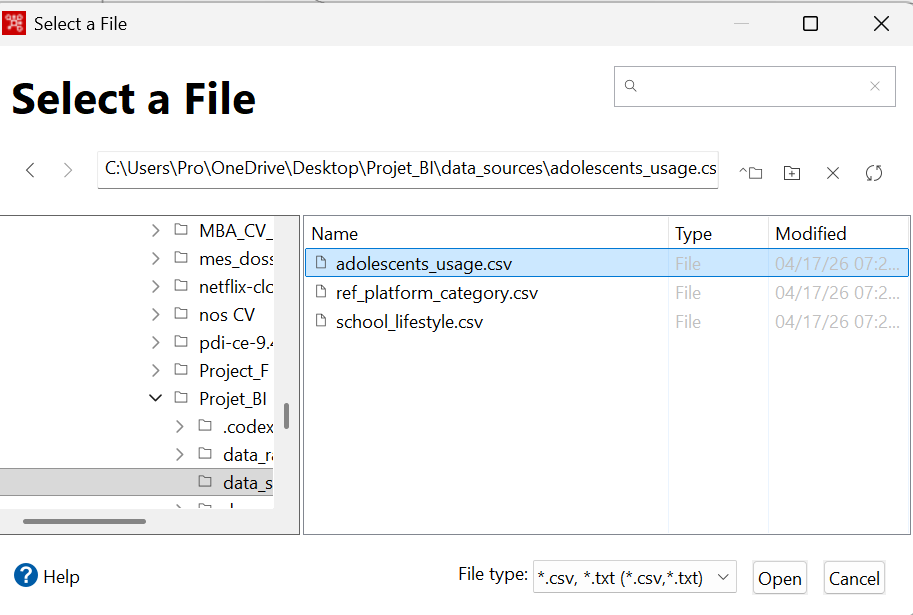
\includegraphics[width=\linewidth,height=0.27\textheight,keepaspectratio]{figures/fig_02_staging_csv.png}
  \caption{Paramétrage d'une extraction CSV.}
\end{subfigure}\hfill
\begin{subfigure}{0.48\linewidth}
  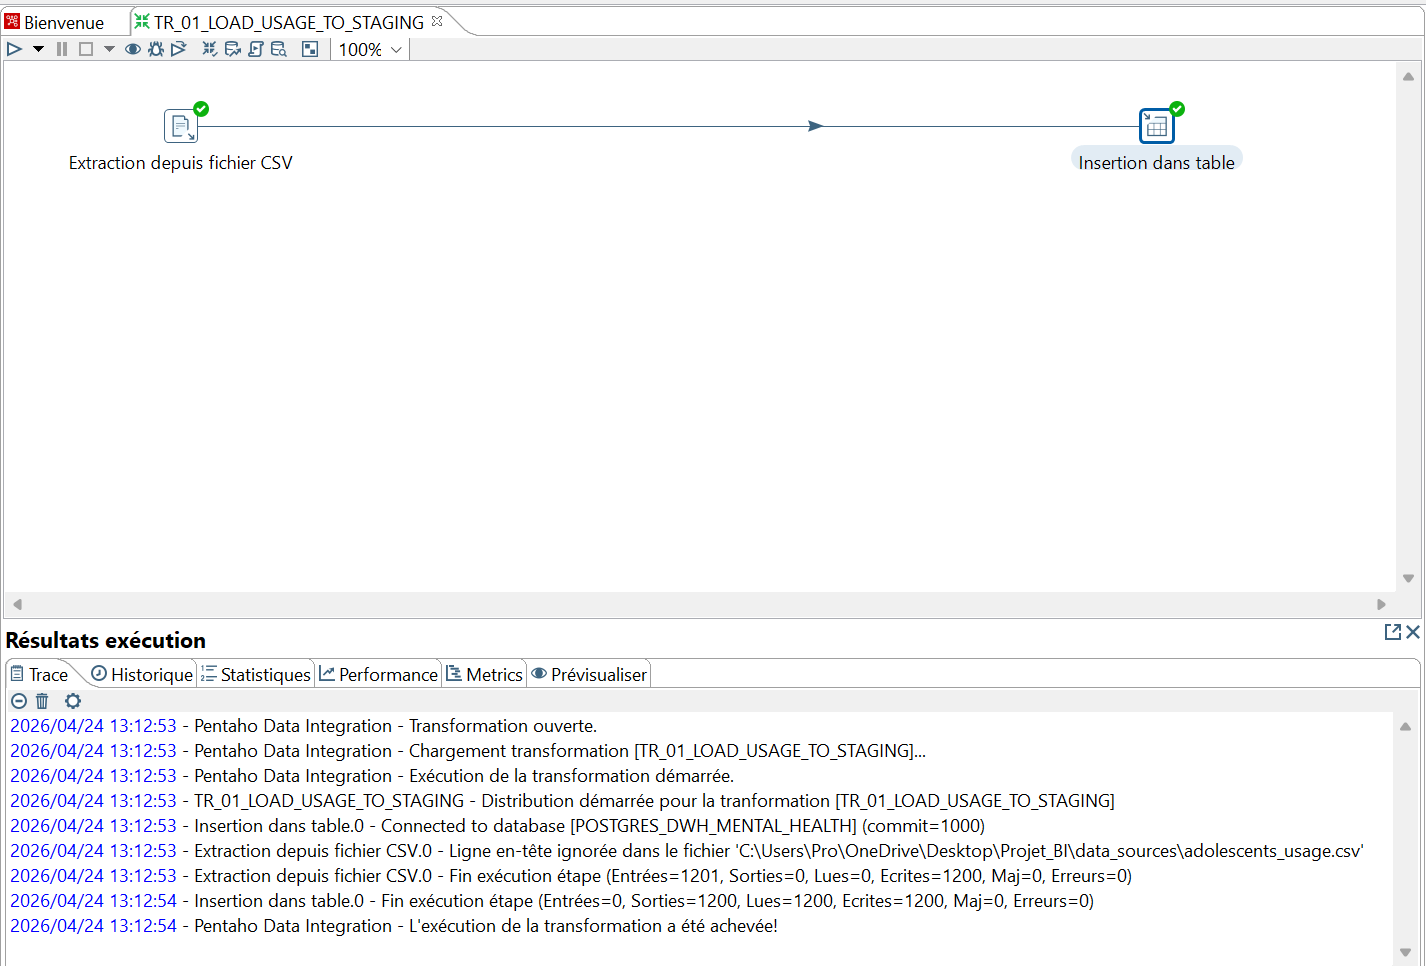
\includegraphics[width=\linewidth,height=0.27\textheight,keepaspectratio]{figures/fig_03_staging_success.png}
  \caption{Exécution réussie d'un chargement staging.}
\end{subfigure}
\caption{Exemple d'alimentation d'une table staging à partir d'un fichier CSV.}
\end{figure}

\begin{figure}[H]
\centering
\begin{subfigure}{0.48\linewidth}
  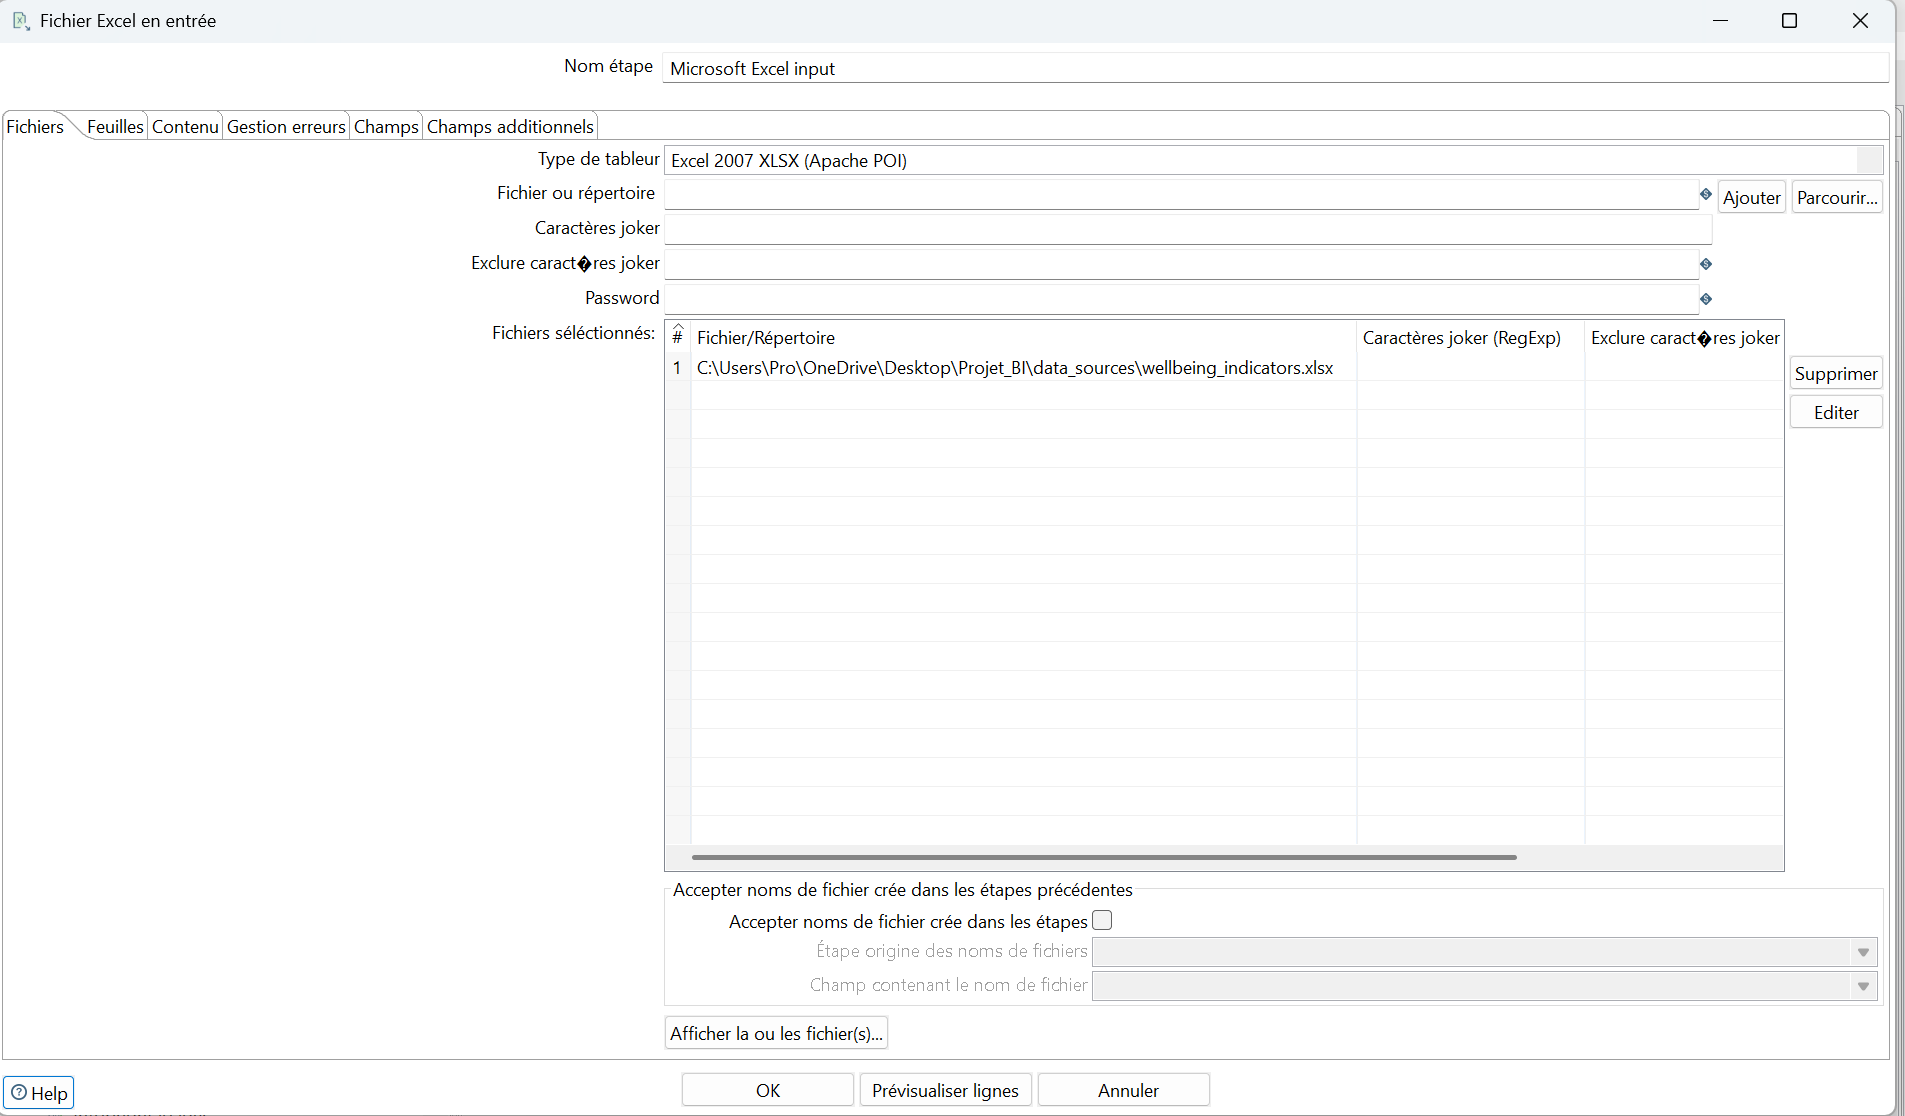
\includegraphics[width=\linewidth,height=0.27\textheight,keepaspectratio]{figures/fig_04_excel_input.png}
  \caption{Configuration de l'entrée Excel.}
\end{subfigure}\hfill
\begin{subfigure}{0.48\linewidth}
  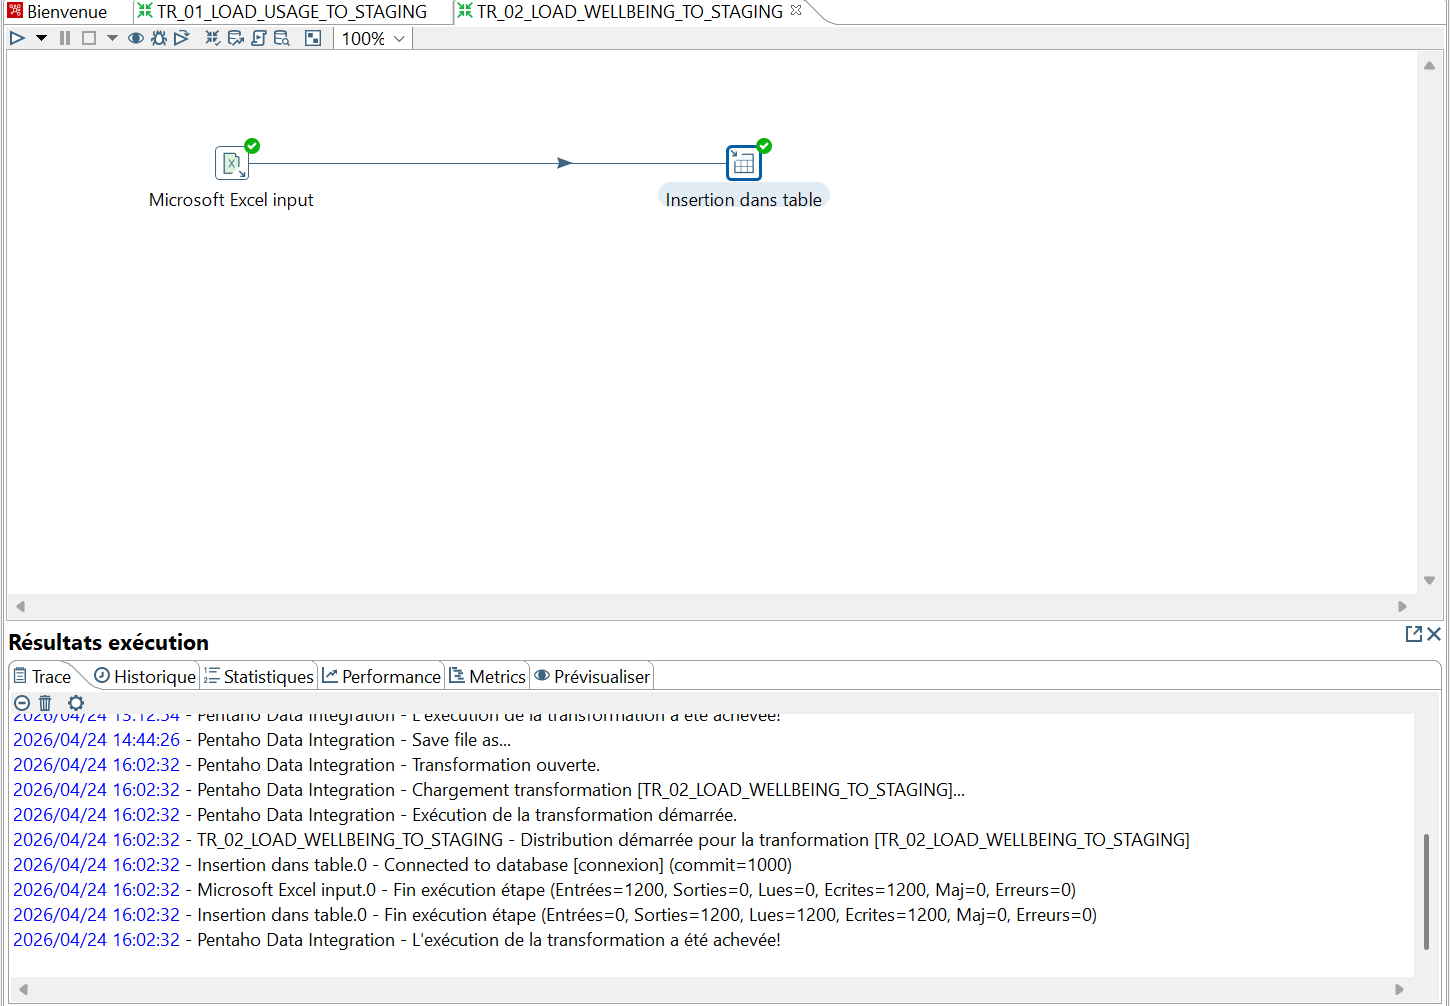
\includegraphics[width=\linewidth,height=0.27\textheight,keepaspectratio]{figures/fig_05_excel_success.png}
  \caption{Chargement réussi du fichier Excel.}
\end{subfigure}
\caption{Chargement des indicateurs de bien-être depuis Excel.}
\end{figure}

\section{Construction des dimensions}

Les dimensions sont construites à partir des valeurs distinctes présentes dans les tables de staging. Ce choix évite de créer manuellement les membres de dimensions et garantit l'alignement avec les données réelles.

\begin{figure}[H]
\centering
\begin{subfigure}{0.48\linewidth}
  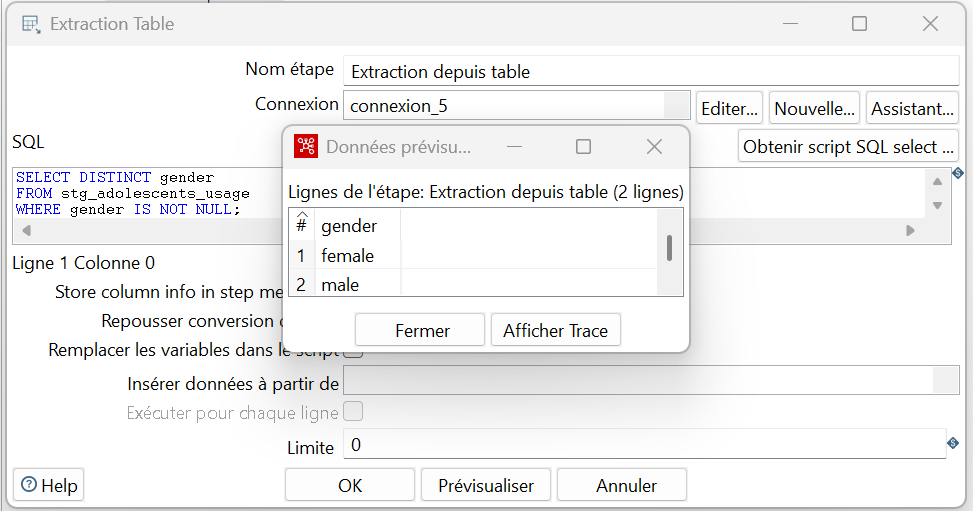
\includegraphics[width=\linewidth,height=0.28\textheight,keepaspectratio]{figures/fig_06_dim_gender.png}
  \caption{Dimension genre depuis les valeurs distinctes.}
\end{subfigure}\hfill
\begin{subfigure}{0.48\linewidth}
  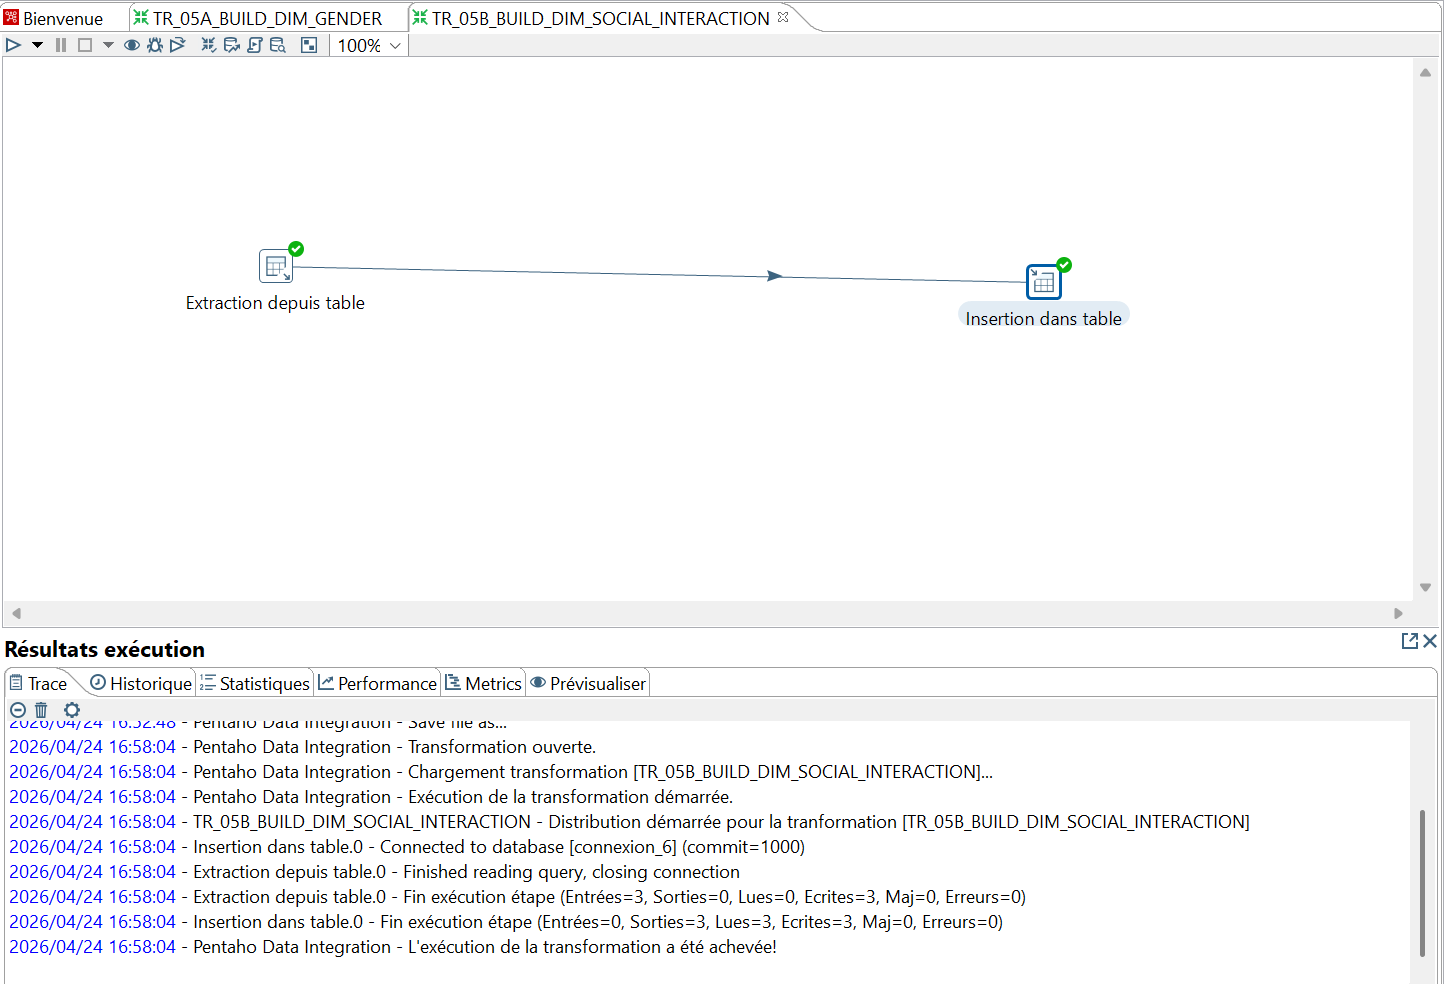
\includegraphics[width=\linewidth,height=0.28\textheight,keepaspectratio]{figures/fig_07_dim_social.png}
  \caption{Dimension interaction sociale.}
\end{subfigure}
\caption{Construction de dimensions simples à partir des tables de staging.}
\end{figure}

\safeimage{0.72}{figures/fig_08_dim_age.png}{Dimension âge avec âge exact et tranche d'âge.}
\safeimage{0.72}{figures/fig_09_dim_platform.png}{Dimension plateforme enrichie par le référentiel des catégories.}

\section{Transformation Avancée 1 : préparation qualité des faits}

La transformation \texttt{TR\_06\_QUALITY\_PREPARE\_FACT} prépare les données propres avant le chargement final. Elle ne charge pas encore la table de faits : elle consolide, contrôle et enrichit les données dans une table intermédiaire \texttt{stg\_fact\_clean}.

\begin{analysisbox}
Cette transformation a un rôle de contrôle qualité. Elle sépare les lignes valides des lignes rejetées, supprime les doublons, transforme un code technique en libellé métier et ajoute une trace du pipeline ETL. Elle rend donc le chargement final plus sûr.
\end{analysisbox}

\begin{landscape}
\safeimage{0.90}{figures/fig_10_tr06.png}{Transformation \texttt{TR\_06\_QUALITY\_PREPARE\_FACT} : contrôle qualité, tri, dédoublonnage, mapping et chargement propre.}
\end{landscape}

\subsection{Logique de traitement}

\begin{enumerate}[label=\textbf{\arabic*.},leftmargin=1.2cm]
  \item extraction des données consolidées depuis les tables de staging ;
  \item création d'un statut qualité et d'une raison de rejet ;
  \item séparation des lignes valides et invalides ;
  \item tri par \texttt{id\_adolescent} puis suppression des doublons ;
  \item mapping de \texttt{depression\_label} vers \texttt{depression\_status} ;
  \item ajout de la constante \texttt{pipeline\_source} pour la traçabilité ;
  \item insertion dans \texttt{stg\_fact\_clean} ;
  \item insertion des lignes rejetées dans \texttt{etl\_reject\_health}.
\end{enumerate}

\begin{codebox}[Exemple de règle de validation logique]
\begin{lstlisting}[style=sqlstyle]
CASE
  WHEN age IS NULL THEN 'Age manquant'
  WHEN stress_level NOT BETWEEN 0 AND 10 THEN 'Stress invalide'
  WHEN daily_social_media_hours > 24 THEN 'Usage quotidien invalide'
  ELSE 'VALID'
END AS quality_status
\end{lstlisting}
\end{codebox}

\begin{resultbox}
La table \texttt{stg\_fact\_clean} contient 1200 lignes propres. La table de rejet qualité ne contient aucune ligne dans le jeu de données final, ce qui indique que les contrôles configurés ont été validés sur les données disponibles.
\end{resultbox}

\section{Transformation Avancée 2 : lookups des dimensions et chargement de la table de faits}

La transformation \texttt{TR\_07\_LOAD\_FACT\_WITH\_DIM\_LOOKUPS} réalise le passage final vers le schéma en étoile. Les valeurs métier sont remplacées par les clés des dimensions au moyen de recherches en base de données.

\begin{landscape}
\safeimage{0.90}{figures/fig_11_tr07.png}{Transformation \texttt{TR\_07\_LOAD\_FACT\_WITH\_DIM\_LOOKUPS} : récupération des clés de dimensions et chargement final.}
\end{landscape}

\subsection{Correspondances réalisées}

\begin{table}[H]
\centering
\renewcommand{\arraystretch}{1.25}
\begin{tabularx}{\linewidth}{>{\bfseries}p{3.6cm}p{5.0cm}Y}
\toprule
Dimension & Condition de recherche & Clé retournée \\
\midrule
\db{dim_age} & \texttt{age\_exact = age} & \texttt{id\_age} \\
\db{dim_gender} & \texttt{gender = gender} & \texttt{id\_gender} \\
\db{dim_platform} & \texttt{platform\_usage = platform\_usage} & \texttt{id\_platform} \\
\db{dim_social_interaction} & \texttt{social\_interaction\_level = social\_interaction\_level} & \texttt{id\_social\_interaction} \\
\bottomrule
\end{tabularx}
\caption{Lookups réalisés avant l'insertion dans la table de faits.}
\end{table}

\begin{codebox}[Requête d'extraction utilisée au début de TR\_07]
\begin{lstlisting}[style=sqlstyle]
SELECT
    id_adolescent,
    ((id_adolescent - 1) % 7) + 1 AS id_temps,
    age,
    gender,
    platform_usage,
    social_interaction_level,
    daily_social_media_hours,
    screen_time_before_sleep,
    sleep_hours,
    academic_performance,
    physical_activity,
    stress_level,
    anxiety_level,
    addiction_level,
    depression_label
FROM stg_fact_clean;
\end{lstlisting}
\end{codebox}

\safeimage{0.78}{figures/fig_12_fact_success.png}{Validation du chargement de la table de faits après correspondance avec les dimensions.}

\subsection{Validation SQL}

Les requêtes de contrôle suivantes ont été utilisées pour confirmer que la table de faits est correctement alimentée.

\begin{codebox}[Contrôles SQL finaux]
\begin{lstlisting}[style=sqlstyle]
SELECT COUNT(*) FROM fait_sante_mentale;
-- Résultat attendu : 1200

SELECT COUNT(*) AS lignes_problematiques
FROM fait_sante_mentale
WHERE id_temps IS NULL
   OR id_age IS NULL
   OR id_gender IS NULL
   OR id_platform IS NULL
   OR id_social_interaction IS NULL;
-- Résultat attendu : 0
\end{lstlisting}
\end{codebox}

\begin{resultbox}
La table \db{fait_sante_mentale} contient 1200 observations. Les clés étrangères vers les dimensions sont présentes, ce qui confirme la cohérence du schéma en étoile.
\end{resultbox}
\clearpage % <-- pour sauter une section
\section{Problèmes rencontrés et corrections}

Les difficultés rencontrées ont été traitées de manière méthodique. Elles constituent une partie importante du projet car elles montrent la capacité à diagnostiquer un pipeline décisionnel.

\begin{table}[H]
\centering
\renewcommand{\arraystretch}{1.25}
\small
\begin{tabularx}{\linewidth}{>{\bfseries}p{3.5cm}Y Y}
\toprule
Problème & Cause & Correction appliquée \\
\midrule
Lecture Excel impossible & Type de fichier configuré en ancien format Excel 97--2003 alors que le fichier était en \texttt{xlsx}. & Sélection du type \texttt{Excel 2007 XLSX (Apache POI)}. \\
Bouton de récupération des champs indisponible & Le lien entre étapes n'était pas correctement reconnu ou les métadonnées n'étaient pas propagées. & Activation du lien et récupération des champs depuis l'étape précédente. \\
Erreur de \texttt{TRUNCATE} sur une dimension & La dimension était référencée par la table de faits via une clé étrangère. & Vidage préalable de la table de faits ou désactivation du \texttt{TRUNCATE} sur la dimension. \\
Rejets incorrects dans TR\_07 & Orientation du filtre ou propagation de condition mal interprétée. & Vérification SQL des clés, correction du filtre et validation finale par \texttt{COUNT(*)}. \\
\bottomrule
\end{tabularx}
\caption{Synthèse des problèmes techniques et corrections.}
\end{table}

% ---- Resoudre le probleme dans la table de matiere ----
\addtocontents{toc}{\protect\newpage}
% =====================================================
\chapter{Tableaux de bord Power BI}

\section{Mesures analytiques principales}

Les pages Power BI reposent sur des mesures DAX simples et lisibles. Elles permettent de suivre l'état général du jeu de données et d'analyser les indicateurs par dimension.

\begin{codebox}[Exemples de mesures DAX]
\begin{lstlisting}[style=plaincode]
Total Observations =
COUNTROWS('public fait_sante_mentale')

Stress Moyen =
AVERAGE('public fait_sante_mentale'[stress_level])

Anxiete Moyenne =
AVERAGE('public fait_sante_mentale'[anxiety_level])

Addiction Moyenne =
AVERAGE('public fait_sante_mentale'[addiction_level])

Taux Depression % =
AVERAGE('public fait_sante_mentale'[depression_label]) * 100

Score Risque Mental =
DIVIDE([Stress Moyen] + [Anxiete Moyenne] + [Addiction Moyenne], 3)
\end{lstlisting}
\end{codebox}
\clearpage % <-- pour sauter une section
\section{Page 1 : vue d'ensemble}

La première page présente les indicateurs globaux et deux premières lectures : répartition des observations par genre et stress moyen par plateforme.

\safeimage{0.88}{figures/fig_13_bi_overview.png}{Page Power BI « Vue d'ensemble ».}

\begin{analysisbox}
Cette page joue le rôle de synthèse exécutive. Elle permet de répondre rapidement aux questions suivantes : combien d'observations sont analysées, quel est le niveau moyen de stress, d'anxiété et d'addiction, et comment les observations se répartissent par genre et plateforme.
\end{analysisbox}
\clearpage % <-- pour sauter une section
\section{Page 2 : analyse par plateforme}

La deuxième page compare les indicateurs selon la plateforme utilisée : stress moyen, taux de dépression et addiction moyenne.

\safeimage{0.88}{figures/fig_14_bi_platform.png}{Page Power BI « Analyse par plateforme ».}

\begin{notebox}
Cette page est utile pour observer si certains usages numériques sont associés à des niveaux plus élevés de stress, d'addiction ou de dépression. Les segments par genre et tranche d'âge facilitent l'analyse comparative.
\end{notebox}
\clearpage % <-- pour sauter une section
\section{Page 3 : genre et interaction sociale}

Cette page croise les dimensions \texttt{gender}, \texttt{platform\_usage} et \texttt{social\_interaction\_level}. Elle permet d'identifier des écarts entre groupes.

\safeimage{0.88}{figures/fig_15_bi_gender_social.png}{Page Power BI « Genre et interaction sociale ».}

\section{Page 4 : risque mental et évolution temporelle}

La quatrième page introduit des indicateurs synthétiques : score de risque mental, taux de stress élevé et taux de dépression. Elle ajoute aussi une lecture par tranche d'âge et par trimestre/mois.

\safeimage{0.88}{figures/fig_16_bi_risk_time.png}{Page Power BI « Risque mental et temporalité ».}

\section{Page 5 : sommeil et usage numérique}

La dernière page se concentre sur le sommeil, le temps d'écran avant sommeil et l'intensité d'usage numérique.

\safeimage{0.88}{figures/fig_17_bi_sleep_usage.png}{Page Power BI « Sommeil et usage numérique ».}

\begin{analysisbox}
Cette page complète l'analyse en reliant les habitudes numériques aux variables de sommeil. Elle est pertinente car le sommeil est un facteur explicatif important lorsqu'on analyse les niveaux de stress, d'anxiété ou d'addiction.
\end{analysisbox}

% =====================================================
\chapter{Validation globale et qualité du travail}

\section{Cohérence du pipeline}

Le pipeline final est cohérent car chaque étape a une responsabilité claire.

\begin{table}[H]
\centering
\renewcommand{\arraystretch}{1.25}
\begin{tabularx}{\linewidth}{>{\bfseries}p{4.2cm}Y}
\toprule
Étape & Validation obtenue \\
\midrule
Staging & Les fichiers sources ont été chargés dans des tables PostgreSQL séparées. \\
Dimensions & Les dimensions ont été créées depuis les valeurs distinctes ou les référentiels utiles. \\
Préparation qualité & \texttt{stg\_fact\_clean} contient 1200 lignes propres. \\
Chargement final & \db{fait_sante_mentale} contient 1200 observations. \\
Power BI & Les pages exploitent les mesures de la table de faits et les axes des dimensions. \\
\bottomrule
\end{tabularx}
\caption{Validation fonctionnelle de la chaîne décisionnelle.}
\end{table}
\clearpage % <-- pour sauter une section
\section{Apport décisionnel}

La solution permet de répondre à des questions analytiques concrètes :

\begin{itemize}[leftmargin=1.2cm]
  \item quel est le niveau moyen de stress, d'anxiété et d'addiction des adolescents ?
  \item quelles plateformes sont associées aux scores les plus élevés ?
  \item existe-t-il des différences selon le genre ou la tranche d'âge ?
  \item comment le sommeil et le temps d'écran avant sommeil se comportent-ils selon les groupes ?
  \item quels segments nécessitent une attention particulière dans l'analyse du risque mental ?
\end{itemize}

\section{Points forts du projet}

\begin{notebox}
Les points forts sont : une séparation claire staging / dimensions / faits, deux transformations ETL complexes et justifiées, des contrôles SQL de validation, des tables de rejet, des mesures DAX orientées décision et des tableaux de bord organisés par angle d'analyse.
\end{notebox}

% =====================================================
\chapter*{Conclusion et synthèse}
\addcontentsline{toc}{chapter}{Conclusion et synthèse}

Ce projet a permis de réaliser une chaîne décisionnelle complète, depuis les fichiers sources jusqu'aux tableaux de bord Power BI. Les données ont d'abord été importées dans des tables de staging PostgreSQL, puis transformées avec Pentaho Data Integration afin de produire un modèle analytique structuré autour d'une table de faits et de plusieurs dimensions.

Les deux transformations avancées constituent le coeur technique du projet. La première assure la préparation qualité des données : filtrage, dédoublonnage, mapping métier et traçabilité. La seconde réalise les recherches dans les dimensions et charge la table de faits finale. Les validations SQL confirment que la table \db{fait_sante_mentale} contient 1200 observations exploitables.

Enfin, les tableaux de bord Power BI transforment le modèle en outil d'analyse. Les pages réalisées couvrent une vue globale, une analyse par plateforme, une analyse croisée genre / interaction sociale, un suivi du risque mental et une lecture centrée sur le sommeil et l'usage numérique.

\begin{resultbox}
La solution finale est cohérente, professionnelle et défendable : elle respecte la logique d'un Data Warehouse, documente les choix de modélisation, démontre des transformations ETL avancées et fournit des visualisations analytiques directement exploitables.
\end{resultbox}

% =====================================================
\appendix
\chapter{Annexes techniques}

\section{Requêtes de contrôle utiles}

\begin{codebox}[Contrôles PostgreSQL]
\begin{lstlisting}[style=sqlstyle]
-- Contrôle de la table propre
SELECT COUNT(*) FROM stg_fact_clean;

-- Contrôle de la table de faits
SELECT COUNT(*) FROM fait_sante_mentale;

-- Vérification des clés étrangères non nulles
SELECT COUNT(*) AS lignes_problematiques
FROM fait_sante_mentale
WHERE id_temps IS NULL
   OR id_age IS NULL
   OR id_gender IS NULL
   OR id_platform IS NULL
   OR id_social_interaction IS NULL;
\end{lstlisting}
\end{codebox}
\clearpage % <-- pour sauter une section
\section{Principe de chargement de la table de faits}

\begin{codebox}[Principe SQL équivalent aux lookups]
\begin{lstlisting}[style=sqlstyle]
SELECT
    t.id_temps,
    a.id_age,
    g.id_gender,
    p.id_platform,
    s.id_social_interaction,
    f.daily_social_media_hours,
    f.screen_time_before_sleep,
    f.sleep_hours,
    f.academic_performance,
    f.physical_activity,
    f.stress_level,
    f.anxiety_level,
    f.addiction_level,
    f.depression_label
FROM stg_fact_clean f
JOIN dim_temps t
    ON t.id_temps = ((f.id_adolescent - 1) % 7) + 1
JOIN dim_age a
    ON a.age_exact = f.age
JOIN dim_gender g
    ON g.gender = f.gender
JOIN dim_platform p
    ON p.platform_usage = f.platform_usage
JOIN dim_social_interaction s
    ON s.social_interaction_level = f.social_interaction_level;
\end{lstlisting}
\end{codebox}


\end{document}
